% !TeX root = ./pf2023.tex

%\includeonlyframes{current}

\section*{Static data and functions}

\begin{frame}[fragile]{Non-local objects}

  \begin{columns}
    \begin{column}{.75\textwidth}
      \begin{itemize}
      \item Objects can be created outside a function block
        \begin{codeblock}<2->{
#include <random>

std::default_random_engine eng;

auto seed_rand(int s) \{ eng.seed(s); \}
auto get_rand()       \{ return eng(); \}
auto print_rand()     \{ std::cout << get_rand(); \}}\end{codeblock}

      \item<2-> \code{eng} above is a \textit{global} variable
      \item<3-> They have \textit{static} storage duration, i.e. they live for the
        whole program duration
      \item<3-> They live in the \textbf{Static Data} memory segment
      \item<4-> They are initialized before \code{main} is called and destroyed
        after \code{main} has finished
      \end{itemize}

    \end{column}
    \begin{column}{.25\textwidth}<3->
      \centering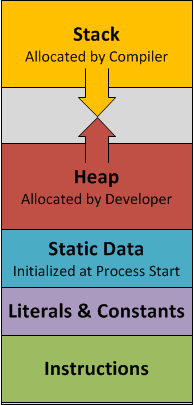
\includegraphics[height=.5\textheight]{images/process-memory-layout}
    \end{column}
  \end{columns}
\end{frame}

\begin{frame}[fragile]{Non-local objects \insertcontinuationtext}
  \begin{itemize}
  \item<1-> Initialization
    \begin{itemize}
    \item Memory for non-local variables is guaranteed to be at least
      initialized to all zeroes
    \item They may be initialized to a constant value known at compile time
    \item They may be initialized dynamically at runtime, e.g. with the result
      of a function call
    \end{itemize}
  \item<2-> Warning
    \begin{itemize}
    \item Non-local variables make reasoning about the program more difficult
      because they encourage to work by side effects
    \item The order of initialization and destruction is deterministic only in
      the same translation unit
    \item \alert{Better avoid them}, especially if mutable (i.e. non constant)
    \end{itemize}
  \end{itemize}
\end{frame}

\begin{frame}[fragile]{Constants}

  \begin{itemize}
  \item One useful application of non-local variables is to define constants,
    possibly inside a namespace
    \begin{codeblock}{
namespace std::numbers \{
  inline constexpr double e  = \ddd ;
  inline constexpr double pi = \ddd ;
  \ddd
\}
}\end{codeblock}
    \item<2-> \code{inline} means that there is only one object in the whole
      program (like for function definitions)
      \begin{itemize}
      \item<2-> to be used if the definitions are in a header file
      \end{itemize}
    \item<2-> \code{constexpr} guarantees that the initialization can be done at
      compile time
    \begin{itemize}
    \item<2-> possibly through the execution of a \textit{constexpr} function
      (not further discussed)
    \item<2-> it implies \code{const}
    \end{itemize}
  \item<3->Of course constants can be defined locally as well
  \end{itemize}

\end{frame}

\begin{frame}[fragile]{Class \code{static} data members}

  \begin{itemize}
  \item<1-> A class data member declared \alert{\code{static}} is not part of
    any object of that class
  \item<2-> A static data member
    \begin{itemize}
    \item<2-> exists even if there are no objects of that class
    \item<3-> has static storage duration
    \item<4-> is defined out-of-class \ldots
    \item<5-> \ldots unless it's declared \code{inline} (C++17) or
      \code{constexpr} (which implies \code{inline}) or is a \code{const}
      integral type
    \end{itemize}
    \vskip -.5cm
    \begin{columns}[t]<4->
      \begin{column}{.5\textwidth}<4->
        \begin{codeblock}<4->{
struct X \{
  static int n;
\};
// probably in a .cpp file
int X::n = 42;}\end{codeblock}
      \end{column}
      \begin{column}{.5\textwidth}
        \begin{codeblock}<5->{
struct X \{
  inline static int n = 42;
\};}\end{codeblock}
      \end{column}
    \end{columns}
  \end{itemize}

\end{frame}

\begin{frame}[fragile]{Class \code{static} data members \insertcontinuationtext}

  \begin{itemize}
  \item A static data member is usually accessed using the scope operator
    \code{::}

    \begin{codeblock}
class std::chrono::system_clock \{
 public:
  static constexpr bool is_steady = \ddd ;
  \ddd
\};

std::cout << std::chrono::system_clock\alert{::}is_steady;\end{codeblock}

  \item But if there is an object of that type, one can use the \code{.} operator
    on that object

    \begin{codeblock}
std::chrono::system_clock clock;
std::cout << clock\alert{.}is_steady;\end{codeblock}

  \end{itemize}
\end{frame}

\begin{frame}[fragile]{Class \code{static} member functions}

  \begin{itemize}
  \item A class member function declared \alert{\code{static}} is not associated
    with any object of that class
  \item They are similar to normal functions, but defined in the scope of a
    class, so that they can access the other members
  \item A static member function can access static data members, but cannot
    access non-static data members
    \begin{itemize}
    \item It cannot be declared as \code{const}
    \end{itemize}
  \end{itemize}
  \begin{codeblock}
class std::chrono::system_clock \{
 public:
  static time_point now() \{ \ddd \}
  \ddd
\};
// system_clock::now() could also be defined out-of-class\end{codeblock}
    \begin{codeblock}
using namespace std::chrono_literals;
std::this_thread\alert{::}sleep_until(std::chrono::system_clock\alert{::}now() + 15ms);\end{codeblock}

\end{frame}
